\documentclass[11pt,a4paper]{article}

% ---------------------------------------------------------------------------
% Packages
% ---------------------------------------------------------------------------
\usepackage[T1]{fontenc}
\usepackage[utf8]{inputenc}
\usepackage{lmodern}
\usepackage{microtype}
\usepackage[a4paper,margin=2.15cm]{geometry}
\usepackage{graphicx}
\usepackage{booktabs}
\usepackage{array}
\usepackage{caption}
\usepackage{subcaption}
\usepackage{float}
\usepackage{xcolor}
\usepackage{enumitem}
\usepackage{titlesec}
\usepackage{titling}
\usepackage{tikz}
\usetikzlibrary{positioning,arrows.meta}
\usepackage[hidelinks]{hyperref}

% ---------------------------------------------------------------------------
% Layout tuning
% ---------------------------------------------------------------------------
\setlength{\droptitle}{-1.5cm}
\setlength{\parskip}{0.26em}
\setlength{\parindent}{0pt}
\captionsetup{font=small,labelfont=bf}
\titlespacing*{\section}{0pt}{0.9em}{0.35em}
\titlespacing*{\subsection}{0pt}{0.6em}{0.25em}
\titleformat{\section}{\large\bfseries}{\thesection}{0.6em}{}
\titleformat{\subsection}{\normalsize\bfseries}{\thesubsection}{0.6em}{}
\setlist[itemize]{leftmargin=1.2em,topsep=2pt,itemsep=1pt}

\newcommand{\code}[1]{\texttt{\small #1}}

% ---------------------------------------------------------------------------
% Title page
% ---------------------------------------------------------------------------
\newcommand{\studentrow}[2]{#1 & \texttt{#2}\\}

\begin{document}

\begin{titlepage}
\centering
\vspace*{0.6cm}

{\Large NOVA IMS\\[0.15cm]
Master in Data Science and Advanced Analytics\par}

\vspace{1.2cm}
{\rule{0.82\textwidth}{0.5pt}\par}
\vspace{0.9cm}

{\Huge\bfseries Predicting FIFA Player Overall Rating\par}
\vspace{0.35cm}
{\Large An End-to-End MLOps Pipeline on the European Soccer Database\par}

\vspace{0.9cm}
{\rule{0.82\textwidth}{0.5pt}\par}

\vfill

\begin{minipage}{0.72\textwidth}
\centering
{\large\bfseries Group Members\par}
\vspace{0.35cm}
\renewcommand{\arraystretch}{1.18}
\begin{tabular}{@{}>{\raggedright\arraybackslash}p{0.58\textwidth}r@{}}
\toprule
\textbf{Name} & \textbf{Student No.} \\
\midrule
\studentrow{Martim L\'ibano Monteiro}{20250429}
\studentrow{Sim\~ao Jos\'e}{20250410}
\studentrow{Francisco Henriques}{20250417}
\studentrow{Pedro Carrasqueira}{20250488}
\studentrow{Ant\'onio Parafita}{20250363}
\bottomrule
\end{tabular}
\end{minipage}

\vfill

{\large Machine Learning Operations (MLOps)\par}
\vspace{0.15cm}
{\large 2025/2026\par}

\end{titlepage}


% ===========================================================================
\section{Problem, data and success metrics}
% ===========================================================================
This project builds an MLOps pipeline to predict a football player's FIFA \code{overall\_rating} based on their in-game attributes. The dataset comes from Kaggle's European Soccer Database, a SQLite dump covering 11 European leagues from 2008 to 2016. We mainly rely on the \code{Player\_Attributes} table, which provides about 184,000 player snapshots containing 33 skill ratings (on a 0-100 scale), preferred foot, and work-rate stats. We also joined the \code{Player} table to add height, weight, and birth date.

We chose this dataset because it includes common data engineering issues: missing values, inconsistent categorical fields, date parsing, and a leakage-prone feature that is too close to the target. After cleaning, the valid \code{overall\_rating} values range from 42 to 90. To keep development cycles fast, we run the pipeline on a fixed 6,000-row sample (seed 42) so a full local run completes in a few minutes. The full table can be built on demand with \code{scripts/build\_dataset.py}.

Since the target ratings are bounded and relatively symmetric (mean around 68), we model them directly without any log transformations. We set our baseline success metrics before training, which are evaluated on a held-out test set in Table~\ref{tab:metrics}.

\begin{table}[H]
\centering
\small
\begin{tabular}{@{}llcc@{}}
\toprule
\textbf{Metric} & \textbf{Role} & \textbf{Target (PoC)} & \textbf{Achieved} \\
\midrule
RMSE (pts)            & Primary; penalises large errors        & $\leq 3.0$  & \textbf{1.45} \\
MAE (pts)             & Typical absolute error                  & $\leq 2.5$  & \textbf{1.05} \\
$R^2$                 & Share of rating variance explained      & $\geq 0.85$ & \textbf{0.954} \\
MAPE (\%)             & Relative error for stakeholders         & $\leq 5$    & \textbf{1.57} \\
Within 2 pts (\%)     & How often a prediction is close         & $\geq 70$   & \textbf{86.8} \\
\bottomrule
\end{tabular}
\caption{Success metrics, targets and results. The champion (HistGradientBoosting) meets every
criterion on the held-out test set.}
\label{tab:metrics}
\end{table}

% ===========================================================================
\section{Project planning and pipeline architecture}
% ===========================================================================
The project is implemented as separate Kedro pipelines rather than a single notebook, which makes each stage runnable and testable on its own. The pipeline covers data quality checks, cleaning, feature generation, model training with MLflow tracking, explainability, containerized serving, and drift monitoring. Each part can run independently through Kedro.

We structured the data using Kedro's standard layering (\code{01\_raw} to \code{08\_reporting}). As shown in Figure~\ref{fig:dag}, the architecture consists of eight interconnected pipelines. The data prep stages run sequentially, followed by two parallel branches that use the trained champion model. Running \code{kedro run} executes the entire DAG, but we can also trigger individual components with \code{kedro run -{}-pipeline <name>}. This structure keeps retraining, batch scoring, and drift checks as separate operational tasks: \code{model\_predict} can score new data, and \code{data\_drifts} can check for distribution shifts without needing to retrain the model from scratch.

\begin{figure}[H]
\centering
\begin{tikzpicture}[
  node distance=4mm and 6mm,
  box/.style={draw, rounded corners=2pt, fill=blue!10, font=\footnotesize\ttfamily,
              minimum height=8mm, inner xsep=5pt, align=center},
  arr/.style={-{Stealth[length=2.5mm]}, thick, gray!55}]
  \node[box] (q)  {data\_quality};
  \node[box, right=of q] (c)  {data\_cleaning};
  \node[box, right=of c] (fe) {data\_feat\_\\engeneering};
  \node[box, right=of fe] (s) {data\_split};
  \node[box, below=8mm of s] (sel) {model\_\\selection};
  \node[box, left=of sel] (tr) {model\_train};
  \node[box, below left=8mm and 2mm of tr] (pr) {model\_predict};
  \node[box, below right=8mm and 2mm of tr] (dr) {data\_drifts};
  \draw[arr] (q) -- (c);
  \draw[arr] (c) -- (fe);
  \draw[arr] (fe) -- (s);
  \draw[arr] (s) -- (sel);
  \draw[arr] (sel) -- (tr);
  \draw[arr] (tr) -- (pr);
  \draw[arr] (tr) -- (dr);
\end{tikzpicture}
\caption{Pipeline DAG. The upper row prepares data, \code{model\_selection} and \code{model\_train}
produce the champion, and \code{model\_predict} and \code{data\_drifts} consume it downstream.}
\label{fig:dag}
\end{figure}

A single \code{modeling.py} module holds the full preprocessing and estimator chain, so the model
compared during cross-validation is the same object that is trained and served. The serving layer
calls the same \code{preprocess\_for\_inference} routine as the offline pipeline, which reduces
the risk of training-serving skew. A row-level parity test would make this check explicit by
verifying that both paths produce identical output on the same input.

% ===========================================================================
\section{Results and conclusions}
% ===========================================================================
\subsection{Data exploration and cleaning}
Initial EDA (\code{exploratory\_data\_analysis.ipynb}) on the raw sample guided the preprocessing choices. As shown in Figure~\ref{fig:eda}, the target \code{overall\_rating} is roughly symmetric and bounded, so we modeled it directly without transformation.

\begin{figure}[H]
\centering
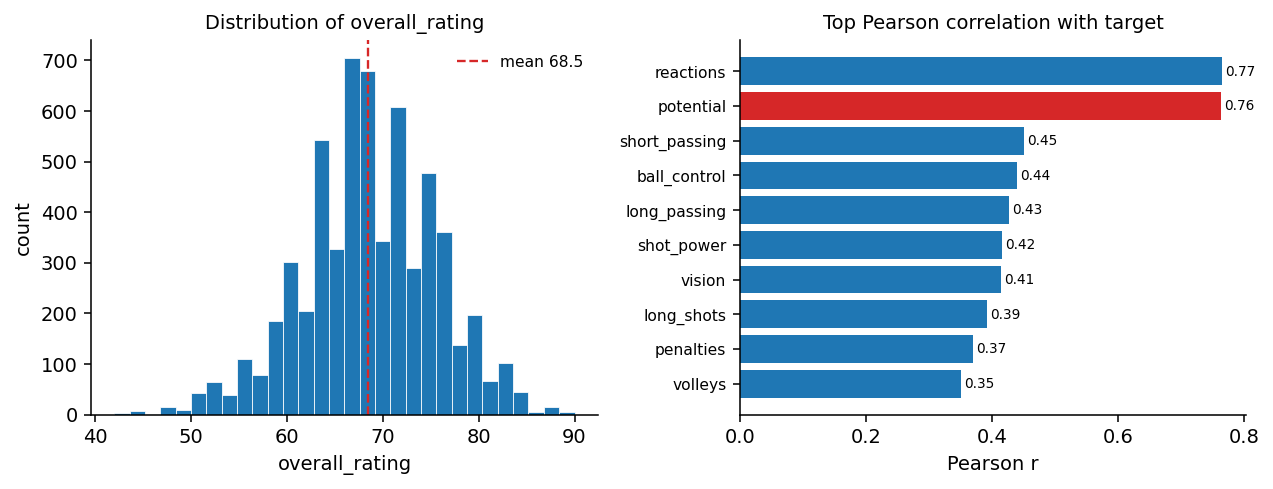
\includegraphics[width=0.78\textwidth]{figures/eda_overview.png}
\caption{Left: Distribution of \code{overall\_rating} (mean 68.5). Right: Top Pearson correlations with the target. Note \code{potential} is highly correlated but must be dropped to prevent target leakage.}
\label{fig:eda}
\end{figure}

The strongest predictor, \code{potential} ($\rho \approx 0.76$), was dropped because it would not be available at inference time in a real-world scouting scenario. For the work-rate features, which contained noisy labels (e.g., \code{norm}, \code{stoc}), we mapped valid inputs to an ordinal scale ($\{0,1,2\}$) and imputed invalid entries with the mode (medium). Missing skill ratings were imputed with the column median, which we saved for use during serving. We also added age, BMI, an \code{is\_goalkeeper} flag, and average ratings by FIFA skill category.

The \code{data\_quality} pipeline validates the raw 6{,}000-row sample against 19 rules (schema, ranges, nulls), which all pass.

\subsection{Modelling and validation}
\label{sec:modelling}
We evaluated four models using 5-fold cross-validation. Table~\ref{tab:cv} shows that tree-based models significantly outperformed linear baselines, indicating strong non-linear interactions between player attributes. We selected HistGradientBoosting as the champion model. On the held-out test set, it achieved an RMSE of 1.45, MAE of 1.05, and an $R^2$ of 0.954.

\begin{table}[H]
\centering
\small
\begin{tabular}{@{}lc@{}}
\toprule
\textbf{Model} & \textbf{CV RMSE (pts)} \\
\midrule
HistGradientBoosting (champion) & \textbf{1.59} \\
Random Forest                   & 1.93 \\
Linear Regression               & 3.29 \\
Ridge                           & 3.30 \\
\bottomrule
\end{tabular}
\caption{Five-fold cross-validated RMSE across candidates (\code{model\_selection\_report.json}).}
\label{tab:cv}
\end{table}

The high $R^2$ is expected because the attributes we used are the underlying components of the official FIFA rating formula. However, because the dataset contains multiple snapshots per player, a standard random split can leak player identity between train and test sets. When we performed a grouped split on \code{player\_api\_id} to strictly separate players, performance only degraded slightly (RMSE 1.54, $R^2$ 0.950, 84.2\% within 2 points), which suggests that the random split was not the only reason for the strong test result.

Diagnostic plots (Figure~\ref{fig:diag}) show well-calibrated predictions through the bulk of the distribution and homoscedastic residuals.

\begin{figure}[H]
\centering
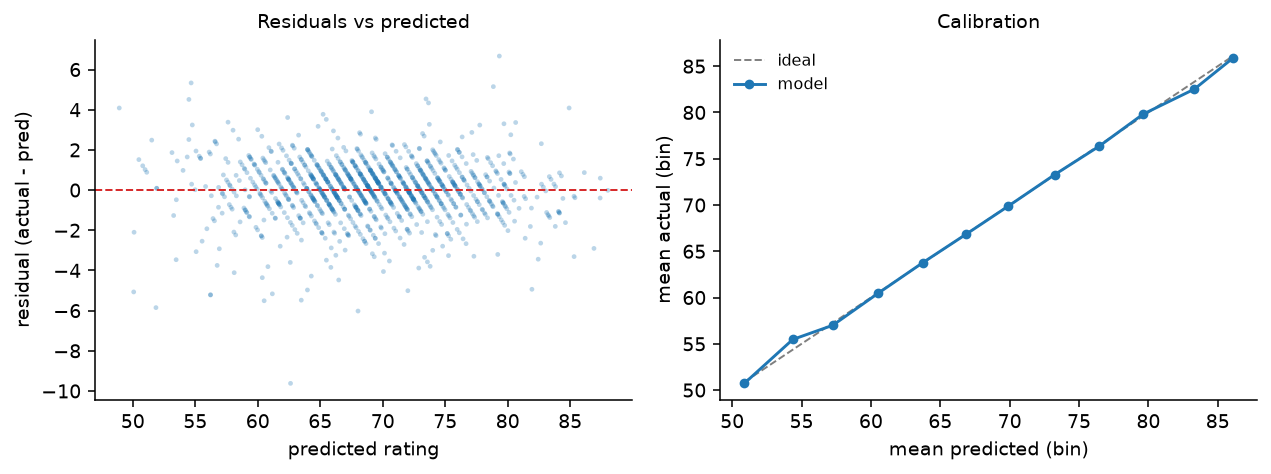
\includegraphics[width=0.78\textwidth]{figures/residuals_calibration.png}
\caption{Left: Residual plot showing no distinct patterns. Right: Binned calibration plot tracking the identity line.}
\label{fig:diag}
\end{figure}

For reproducibility, running the pipeline twice in a clean environment yielded the exact same champion model and test metrics.

\subsection{Explainability (SHAP)}
The \code{model\_train} node generates feature importance metrics using SHAP (falling back to permutation importance if necessary). Figure~\ref{fig:shap} shows the features with the largest contribution to predictions.

\begin{figure}[H]
\centering
\begin{subfigure}{0.49\textwidth}
  \centering
  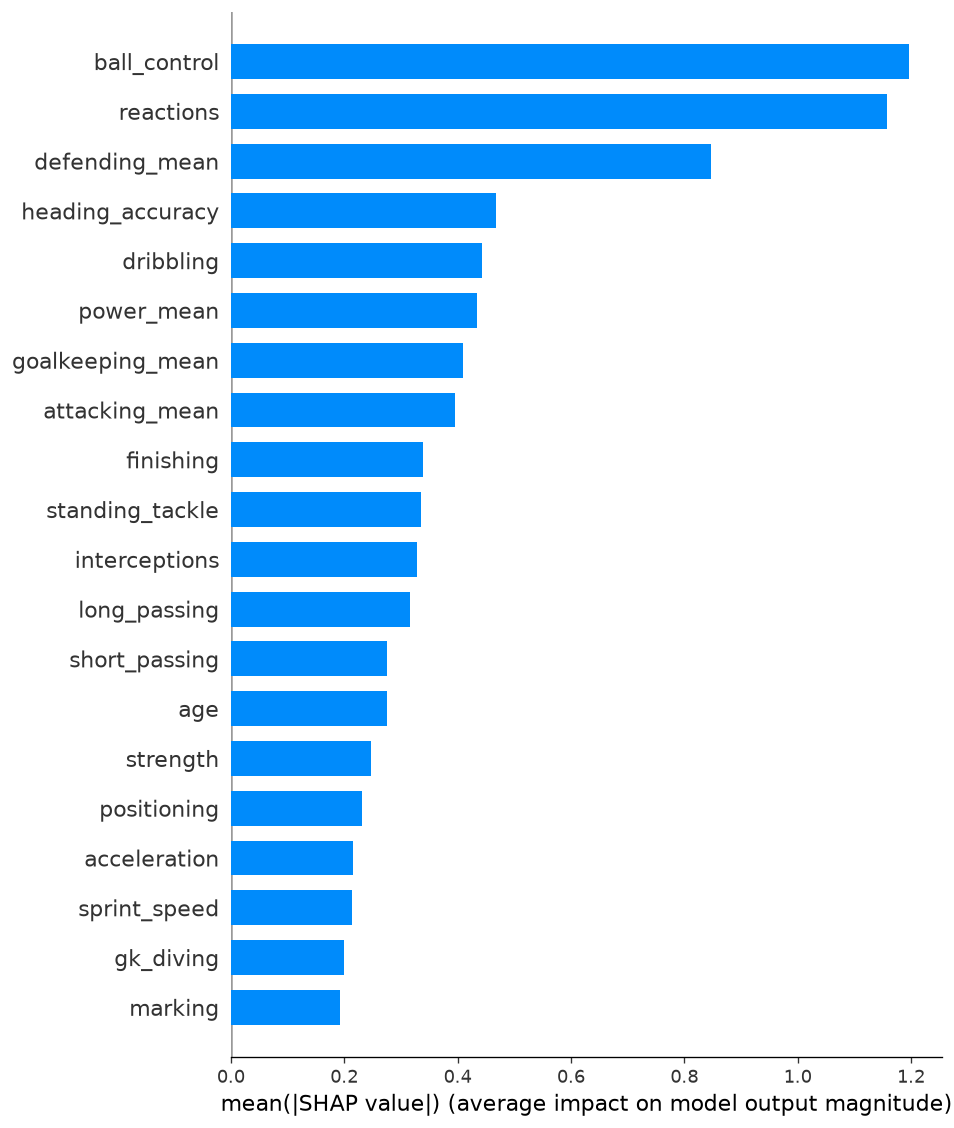
\includegraphics[width=\linewidth]{figures/shap_bar.png}
  \caption{Mean absolute SHAP value.}
  \label{fig:shapbar}
\end{subfigure}\hfill
\begin{subfigure}{0.49\textwidth}
  \centering
  
\includegraphics[width=\linewidth]{figures/shap_summary.png}
  \caption{SHAP summary plot (beeswarm).}
  \label{fig:shapbee}
\end{subfigure}
\caption{Feature explainability. \code{ball\_control} and \code{reactions} are the primary drivers of predictions.}
\label{fig:shap}
\end{figure}

The SHAP summary plot confirms \code{reactions} and \code{ball\_control} are the primary drivers, consistent with our initial EDA. The \code{goalkeeping\_mean} feature separates goalkeeper profiles from outfield-player profiles, so one model can handle both groups.

\subsection{Drift monitoring}
\label{sec:drift}
To detect distribution shifts, the \code{data\_drifts} node compares new batches to the training distribution using Population Stability Index (PSI) and the 2-sample Kolmogorov-Smirnov (KS) test.

The baseline run (\code{drift\_report.json}) flagged 1 out of 48 features. With $\alpha=0.05$, a single flag is within expected false-positive bounds, so no dataset-level drift was triggered. To validate the monitoring logic, we simulated a drift scenario (\code{drift\_report\_simulated.json}), which flagged 18 features and raised a dataset-level alert. Figure~\ref{fig:drift} compares the PSI scores between the clean and drifted batches. The current implementation monitors feature drift only. Target drift and concept drift would require later batches with observed outcomes.

\begin{figure}[H]
\centering
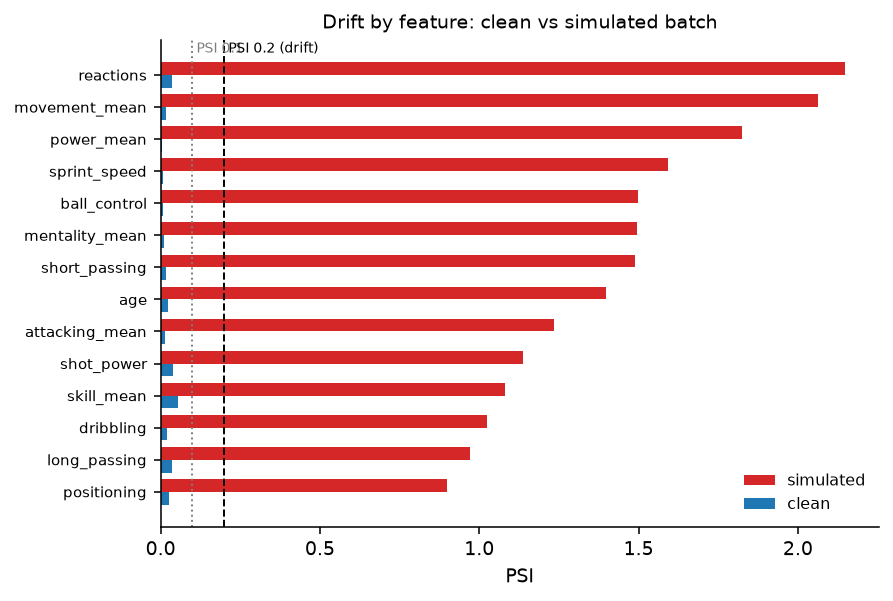
\includegraphics[width=0.54\textwidth]{figures/drift_psi.png}
\caption{Feature-level PSI for the clean batch (blue) and the simulated drift batch (red). The simulated batch crosses the 0.2 PSI threshold for multiple features, triggering a global drift alert.}
\label{fig:drift}
\end{figure}

% ===========================================================================
\section{Future Work \& Production Roadmap}
% ===========================================================================
The current pipeline runs locally on a static CSV sample. Moving it toward production would mainly require changes in orchestration, shared tracking, data validation, storage, and alerting.

\textbf{Next (Immediate upgrades):}
\begin{itemize}
    \item \textbf{Orchestration \& Scheduling:} The Kedro CLI is useful for local runs, but scheduled execution should be handled by an orchestrator. We plan to deploy this via \code{kedro-airflow} so we have proper scheduling and retries.
    \item \textbf{Tracking Server:} Our MLflow setup currently uses a local SQLite file. We need to migrate this to a hosted MLflow server with an object-store backend (like S3) so runs, artifacts, and registered models are shared across the team.
    \item \textbf{Data Quality:} Replace the manual \code{assert} checks with a Great Expectations suite running in CI.
\end{itemize}

\textbf{Later (Scaling up):}
\begin{itemize}
    \item \textbf{Distributed Compute:} Pandas is sufficient for the current 184k-row table, but larger datasets may require porting the pipeline nodes to Spark or Dask.
    \item \textbf{Online Feature Store:} Local Parquet files work for offline training. For real-time serving, we'll need to adopt a feature store like Feast or Hopsworks to handle point-in-time joins and serve features online.
    \item \textbf{Drift Alerting:} The Evidently reports are batch-only right now. We need to set up automated alerting and a retrain trigger when the KS/PSI thresholds are breached.
\end{itemize}

If a clean, independently sourced version of the \code{potential} feature becomes available, the feature store would be the right place to enforce rules to add it back without breaking the current model.

% ===========================================================================
\section{Environment \& Dependencies}
% ===========================================================================
To make the environment reproducible, we pinned all \raisebox{0.5ex}{\~}250 dependencies in \code{requirements-lock.txt}. Rather than listing every package, here are the main packages used by the pipeline:

\begin{itemize}
    \item \textbf{Pipeline \& Data:} \code{kedro} (0.19.x) for orchestrating the DAG, with \code{pandas}, \code{numpy}, and \code{pyarrow} for data wrangling.
    \item \textbf{Modelling \& Metrics:} \code{scikit-learn} (1.x) for the model zoo and preprocessing, with \code{scipy} (1.1x) backing the statistical drift tests.
    \item \textbf{Tracking \& Serving:} \code{mlflow} (3.x) handles the model registry, while \code{fastapi} and \code{uvicorn} run the REST API.
    \item \textbf{Monitoring \& Explainability:} \code{evidently} (0.7.x) generates the HTML drift reports, and \code{shap} (0.5.x) provides feature importance metrics.
    \item \textbf{Testing:} \code{pytest} runs our 25 unit and integration tests.
\end{itemize}

\end{document}